\graphicspath{{mechanism/}}

\chapter{Teaching the Mechanism of the Greenhouse Effect}
\label{chap:mechanism}

As described above, American's lag much of the world regarding acceptance of
anthropogenic climate change. Informally, Michael Ranney,
then other members of our group started questioning whether people were able to
mechanistically explain how human activities cause an increase in global mean
temperature.  Almost no one could provide a satisfactory explanation, including
us! Prof. Ranney, Lloyd Goldwasser, and Daniel Reinholz (along with input from
myself and Ron Cohen) proceeded to develop a short \~400-word description of the
mechanism. This text is reproduced in full in Appendix~\ref{app:400words}.
Before reading the text yourself, I would encourage you to spend 10 minutes
describing \emph{your} understanding either aloud or on paper.\footnote{If you
personally doubt the veracity of anthropogenic climate change, then you may
modify the exercise to describing the mechanism of the greenhouse effect, first
described by Nobel laureate XXX Ahreneous (Sp?) in \citeyear{Ahreneous} (and
accepted as fact since that time!).}

Given that our informal investigations implied that almost no-one knew the basic
concepts described in our 400 words, we initiated the line of research described
below. In these experiments, we sought to formally ask:

\begin{enumerate}
\item Is this lack of understanding for the mechanism of global climate change
    as pervasive as it seemed to be?
\item Does instruction regarding the mechanism of global climate change increase
    individuals' acceptance of the reality of anthropogenic climate change?
\end{enumerate}
Along the way, we additionally considered related aspects of learners’
experiences (the details of which are described below).

The history of educational research would imply that it’s quite difficult to arrive
at definitive answers to big policy qeustions. For example, phonics vs.
whole-word reading has been debated at least since the dawn of the Common Era,
as discussed in \textcite{history-reading-instruction}. Below, however, I report
on a series of experiments that argue strongly (if not definitively!) that
instruction regarding the pysical mechanism of the greenhouse effect appears to
have some positive effect on public acceptance of anthropogenic climate change.
As discussed above, such public acceptance seems central to any truly democratic
approach to the problem of climate change.

\section{Survey methods}
\label{sec:survey}

Chapters~\ref{chap:mechanism}, \ref{chap:evil-ndi}, and \ref{chap:pro-ndi} all
utilize similar survey methods to assess climate-related beliefs and attitudes,
in addition to a number of related constructs relevant to Ranney's
\citeyear{ranney-rtmd} RTMD theory. Here we describe the nature of these
surveys, and our methods for analyzing them. For reference, the full list of
survey items used in this body of research is included in
Appendix~\ref{app:survey-items}.

\section{Clarifying \texorpdfstring{“beliefs”}{"beliefs"} and
    \texorpdfstring{“attitudes”}{"attitudes"}}

Survey methods in the social sciences may use the terms “belief” and “attitude”
in numerous ways. For example, an “attitude” may refer to a measured response,
whereas a “belief” may refer to a latent variable that explains a number of such
responses \cite{some-attitude-latent-var-ref}. Here, we take a more
common-language approach. Specifically, in the text that follows, a “belief” is
a measure of agreement with an objectively verifiable fact about the world (For
example. For example, the reality of anthropogenic climate change (item gw1_2)
may be difficult to ascertain, but in the end, it is something that could be
settled by observation. An “attitude,” on the other hand, is a measure of
agreement with an emotional stance towards some aspect of the world. For
example, worry about global warming (gw2_3).

\section{An overview of survey items}

Primarily taken from Callie’s master’s thesis. The first page in particular was
selected as the most targeted set of 6 questions targeting the 6 RTMD
constructs \cite{ranney-rtmd}.

\textbf{Include the RTMD graph here.}

\section{Na\"ive survey results}

Most of the climate-related interventions that follow include some measure of
participant attitudes and beliefs prior to the intervention. In this thesis, we
report on insights into different forms of \emph{intervention}. Thus, a detailed
consideration of these na\"ive
results is beyond our scope. However, some of the relationships obtained seem
relevant to understanding the mind of our potential students. I thus note such
results below. For a fuller treatment of survey material, please consult the
relevant publications of the Reasoning group
\cite[notably,][]{cohen-thesis,ranney-etal-2012}.

We start by noting that the number of potential relationships between the many
variables we have measured would require an enormous amount of data to test
fully. As such, we will restrict ourselves primarily to the exploration of
\emph{a priori} relationships of interest.

Include multi-correlation figures here.

Evo—GW link
Knowledge / self-knowledge (this isn’t really part of this section)
Other stuff? Maybe nationalism GW link? How does this tie generally into our
theoretical framework? How does it compare and contrast with Ranney’s previous
work?

\section{Acknowledgements}

The work reported in this chapter has been previously published, in part, in
\textcite{ranney_why_inpress,and_others}. It is re-used here with their
permission, and the permission of the publishers.

\section{Experiment 1: Classroom interventions at UC and UT}
\label{sec:mech-classroom}

This experiment was a fairly thick observation of individuals' beliefs,
attitudes and knowledge. We sought to understand how a relatively brief 400-word
mechanistic explanation might affect these measures, as well as how this might
be modulated by prior commitment to one's own explanations and stated attitudes.
The general flow of the experiment is given in Figure~\ref{fig:mech-flow}.

\begin{figure}[h]
    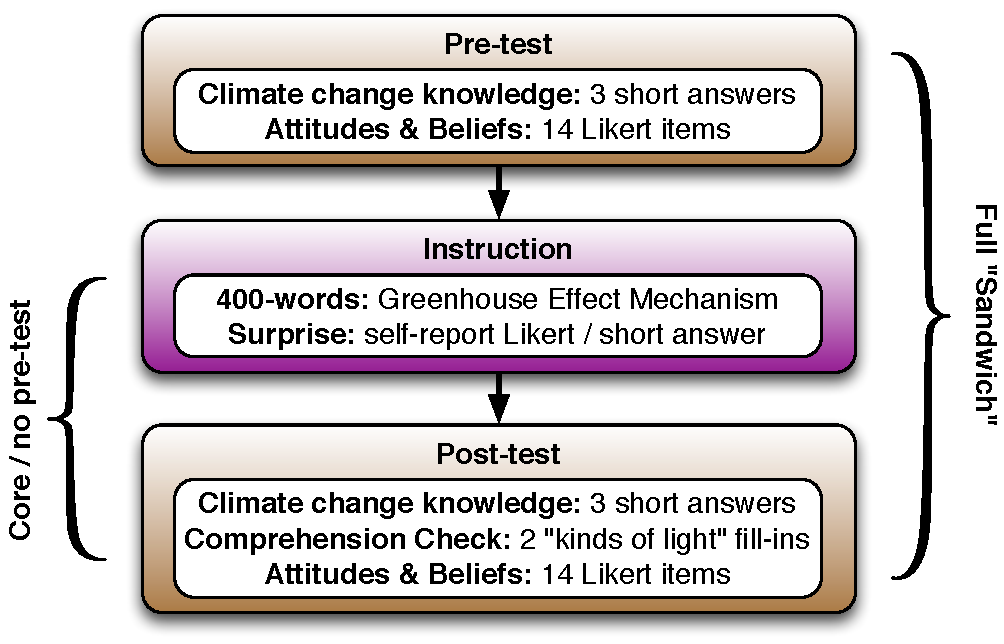
\includegraphics[width=6.5in]{mech-survey-flow1.pdf}
    \caption{An overview of experimental flow for
        Section~\ref{sec:mech-classroom}. Flow for other experiments in
        Chapter~\ref{chap:mechanism} was similar. The analogy to a sandwich
        takes the knowledge and attitutde tests to be slices of bread, and the
        educational intervention itself is the “jam.”}
    \label{fig:mech-flow}
\end{figure}

The primary goal here was a proof of concept. By assessing university
students---some of our nation’s most highly educated citizens---we provide a
strong test of our belief that most Americans are ignorant of the mechanism of
global climate change. An addition concern was that for maximal power, it is
preferable to sample na\"ive beliefs prior to the intervention. In such a
design, we are able to use repeated measures statistics and consequently have
much greater power. On the downside, however, problems can arise from assessment
prior to an intervention. For example, we were concerned that individuals might
exhibit an increase in their stated belief in anthropogenic climate change
merely by dint of experimental demand. This is evaluated via comparison between
our sandwich and no-pretest groups.

As described in Section~\ref{sec:survey}, pre-test responses can be used to
asses na\"ive knowledge and attitudes in the general public. 

% Ryan thinks this is unconvincing, game-show like. Could make a parallel with
% Jame's psychophysical experiments, where people could clearly know that an
% apple is red, but they need to be trained to report the basic visual
% properties of what they see preferentially over reporting "basic level"
% phenomena. The "basic pieces" of our mechanism do indeed seem new to most, but
% we have yet to formally test that part.

\subsection{Experimental Methods}

The general form of the intervention is given in Figure~\ref{fig:mech-flow}.
Participants were split into two groups, receiving either the “no-pretest”
version of the intervention, or the full “sandwich” (filled with nourishing
descriptions of climate change!). The climate change knowledge portion of the
pre- and post-tests consisted of the three questions described in
Section~\ref{sec:materials}. For this experiment, the likert items (all on a 1-9
scale) consisted only of \textsf{knwgbl} followed by the first 13 items in
Table~\ref{table:rtmd-questions}. Both groups read the educational text
regarding the mechanism of greenhouse gasses (reproduced in full in
Appendix~\ref{app:400words}), and indicated any surprise they may have
experienced (again, on a 1-9 scale). The “kinds of light” check consisted of two
fill-in-the-blank questions regarding the kinds of light coming to earth from
the sun and radiating away. Here, “sunlight” or “visible light” were considered
correct for incoming, and “infrared” was considered correct for outgoing.
Some participants wrote “ultraviolet” for incoming light, which one could
charitably ascribe to a partially correct understanding.

In addition to the intervention proper described above, participants also
completed a demographic survey, detailed in Table~\ref{table:demographics}.
The experiment began with a page of instructions, including the assertion that
no tricks or deceptions were involved in this study. Lastly, given that their
experimental intervention was shorter, individuals in the “no pre-test” group
were asked to provide some feedback on the intervention, and also on Al Gore’s
“An Inconvenient Truth” (if they had seen it). These responses were used to
refine our methods going forward, and \textcite{bem-future} notwithstanding,
should have had no effect on the results.

\subsubsection{Participants}

For this intervention, we have collected data from 103 Berkeley undergraduates
in a single class, and 49 from two classes at the University of Texas,
Brownsville. Ages? Gender?

\subsubsection{Procedure}

Participants were run simultaneously for each of the two classes. Instructions
were administered by the course instructor, and students received one of two
packets---placing them into one of the two groups described above. After
completing the consent form on the front of the packet, individuals proceeded to
read and answer questions. The entire experiment required approximately
25 minutes to complete.

\subsubsection{Analysis}

Handwritten responses were coded and placed into a spreadsheet (for details, see
Appendix~\ref{app:coding}. Given the rich nature of these data, many analyses
were employed. As such, please see the results section that follows for details
of the analysis used for each question.

\subsection{Results}

First off, individuals definitely did not have a clear mechanistic understanding
of how greenhouse gases contribute to global warming. Prior to instruction,
\emph{no} participants indicated anything about different kinds of radiation, or
atmospheric retention time for the sun's energy. Afterwards, though,
participants were often able to at least recall some basic details. For example,
40/103 described something about different kinds of radiation and 37/103
explained that energy was retained in the atmosphere. 

Participants shifted on average 14\% closer to ``extreme'' agreement with
climate change items. Combining groups using an imputation approach, this was
significant ($t(72)=2.28, p=.01$). There was no difference between groups on the
post-test. In fact, the open-faced group actually had a slightly greater global
warming acceptance attitude as compared to the sandwich group on average. 

Participants reported greater surprise when they were required to commit to
their own description before instruction ($t(42.1)=1.7, p=.05$). These surprise
ratings were increased from a mean of 2.3 to 3.0 on a 9-point scale. It
surprises us that their ratings are so low in general! Overall, a broad range of
surprise ratings, spanning the scale was observed. Ratings from 7 to 9 were only
observed in the Sandwich condition.

\begin{figure}[h]
    \centering
    \subfloat{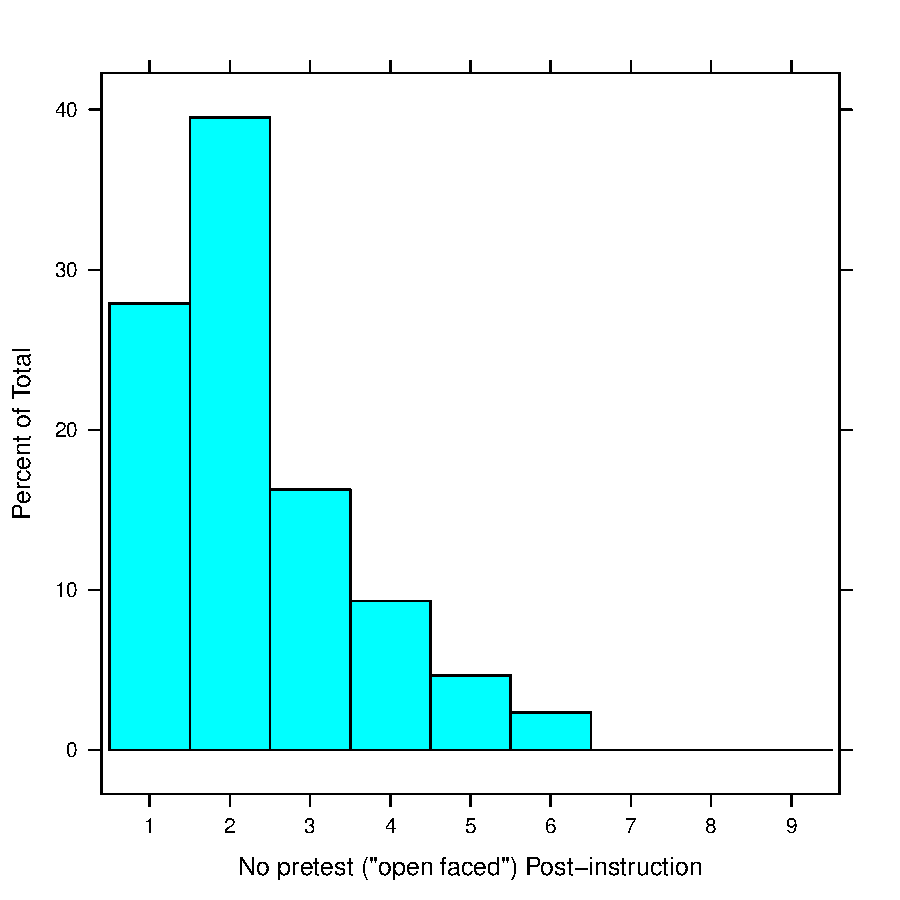
\includegraphics[width=0.5\textwidth]{hypotheses-surprisedistributions1.pdf}}
    \subfloat{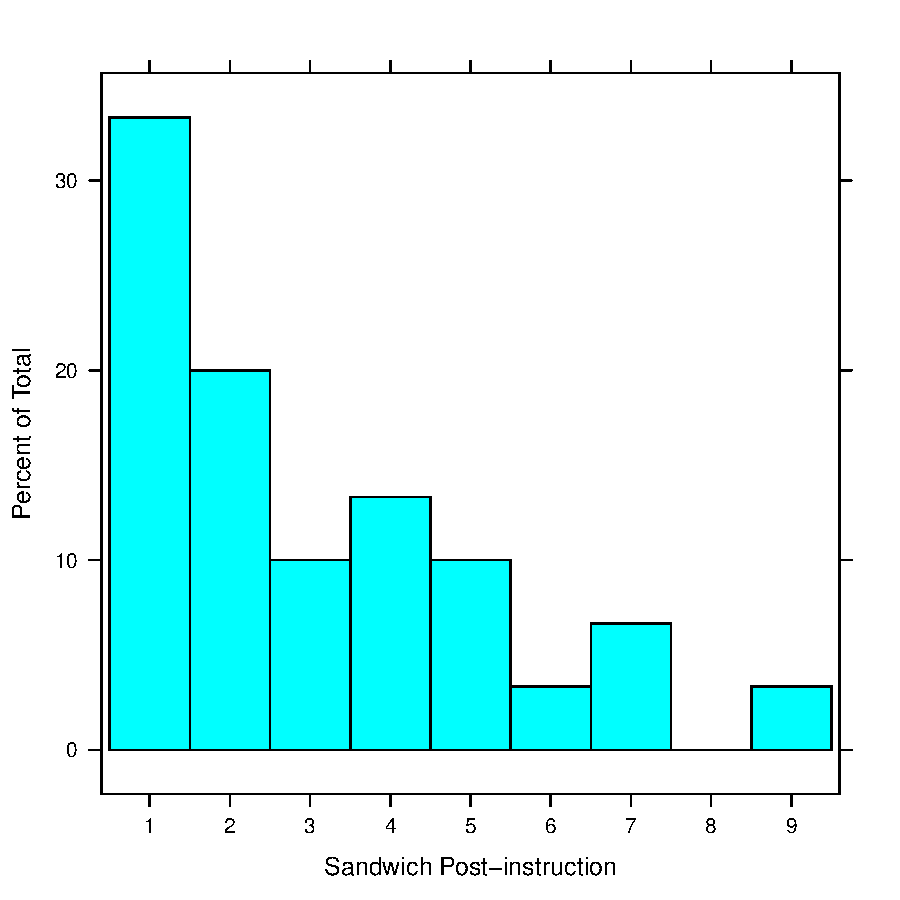
\includegraphics[width=0.5\textwidth]{hypotheses-surprisedistributions2.pdf}}
    \caption{Distributions of surprise ratings for the sandwich and open-faced
        groups, note the slight increase in ``1'' ratings (which may indicate resistance
        to the intervention) co-occurs with an increase (from none) in ratings 7-9 in
        the sandwich group.}
    % For final, re-do these graphs so they have the same y-scales
\end{figure}

Note, I suspect it is unlikely that individuals experienced the same kind of
``visceral'' surprise from the blurb that can be obtained by, for example,
statistics we've used regarding things like abortion and the death penalty. And,
while it may be due to a limitation of imagination, I have difficulty imagining
an evolution item that would elicit this kind of surprise.

In addition, we replicated the relationships predicted by the RTMD theory in
another population. Confirmatory factor analysis yielded quite similar results
to simple correlation tables between the means of attitude-relevant items. In
particular, all proximal relationships held in this population (those
represented by lines in Figure~\ref{fig:rtmd}) and in each survey, either 12 or
13 out of 15 total relationships were in the direction predicted by RTMD. Less
formally, it appears that the correlations between evolution and climate change
increased after our intervention---perhaps indicating a shift in which
participants viewed climate change as part of ``real science.'' Similar
increases in anti-correlation with nationalism were observed. However, we have
not yet established appropriate statistical machinery to test the significance
of these effects.

\subsection{Discussion}

In general, tested university students were largely
ignorant of the mechanism via which greenhouse gases cause global warming,
suggesting that this is a reasonable object of study! More specifically, even
this (relatively dry) 400-word blurb was able to effect shifts in attitudes and
elicit non-trivial surprise ratings from individuals. It remains to see how
attitude shifts and learning are related, but the results as they are seem
sufficient basis for proceeding on an educational research program including
mechanism!


% This should be placed in the correct location above

\begin{figure}
    \begin{center}
        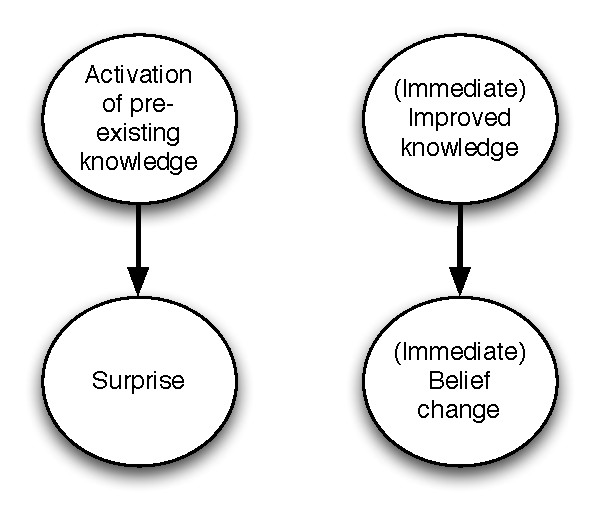
\includegraphics{causal2.pdf}
    \end{center}
    \caption{A graphical model representing the relationship between forms of
        psychological processing of factual information observed in
        chapter~\ref{chap:mechanism}. Here, the relationship between pre-existing
        information and surprise was the result of an experimental manipulation and
        is assumed to be causal.}
    \label{fig:causal-mechanism}
\end{figure}

In addition, we note that there is scant difference between our “sandwich” and
“no pre-test” groups in terms of post-test attitudes. Thus, it seems unlikely
that a pre-test incurs a greater burden of experimental demand over the core
intervention (400 words followed by a post-test). Moreover, in some populations,
the pre-test may help to anchor self assessment (as with our UT data). And
finally, the sandwich intervention appears to increase reported feelings of
surprise, and likely decreases post-hoc bias. Given these many benefits, in the
work that followed, we standardized on using a sandwich style intervention.

\section{A web-based intervention with UC Undergrads}

Given the replicated demonstrations of significant attitude changes described
above, we proceeded to assess whether the mechanism-explanation effects we had
obtained were durable rather than transient. This study extended prior work by
delaying the post-test several days. We also wondered whether an ``experimental
demand'' from the classroom setting might have driven our prior results, so we
provided the intervention on-line; that is, we assessed whether our materials
would elicit significant attitude change even though students participated via
their own computers, without experimenter observation. Thus we concurrently
explored the longevity (via delay) and format (on-line) aspects of our
phenomenon. We also extended our prompts to incorporate more demographic and
introspection queries.

\subsection{Methods}

The survey and instructional materials were those reported in Ranney et
al. (2012a \& 2012b; the latter includes the full 400-word text of our
intervention). The primary difference was that administration was conducted
entirely online, via the Qualtrics Inc. (Provo, UT) system. Eight items were
added to pre- and post-test attitude surveys to add reliability to the related
RTMD metrics (specifically, national and religious affinities; these metrics
will be reported elsewhere). Five further questions were introduced immediately
following the instructional material to elicit introspection (about
embarrassment, disagreement, etc.).  Undergraduates (N=80) were recruited via
the Research Participation Program (RPP), administered by the University of
California, Berkeley (UCB) psychology department. Such recruitment allowed us to
administer a pre-test to about half of the students (38) between 8 and 26 days
($\mu=18.5$ days) before any of the 80 participated in the study, which may have
allayed test-retest effects (although Ranney et al., 2012a, found little
evidence for them). Thus, as with Ranney et al. (2012a), some participants
received the full survey testing ``sandwich'' while others had no pre-test. A
delayed post-test was given to all participants between 1 and 8 days later
($\mu=4$ days). This range was used to assess the timecourse of retention in
planning subsequent studies, We lack the power to test forgetting over time here
(though numerically, did not observe any!).

\subsection{Results and Discussion} 

Split this up! Note results have changed a bit for Knowledge (both kinds) using
regression and glht. Should also do something more definitive with the GW
attitude data (though this was unchanged for the CogSci paper).

In general and as anticipated, we replicated Ranney et
al.’s (2012a) results and extended them by finding that shifts were retained
over the mean (four-day) delay. 
% Include more verbiage here explaining lme4, Anova and glht
Scored knowledge was comparable to previously
tested UC students, rising from 3.8 on pre-test to 6.5 post-test and 6.3 on
followup (gains from pre-test were significant at $p<0.0001$ for both subsequent
scores). GW belief ratings (with higher ratings being
more in concert with science’s consensus) increased from a 6.20 pre-test mean to
a 6.54 post-test mean ($t(79)=2.5, p=0.006$; a healthy improvement on our 1-9
Likert scales!). Some of this improvement
diminished over the following days, but most was retained: the mean score on the
delayed post-test was 6.44 (t(79)=1.7, p=0.05). Self-rated knowledge means
increased markedly from pre- to post-test (4.5 to 5.6 on a 9-point scale,
t(79)=8.5, p<0.001). Retention of this increase, gratifyingly, was also noted on
the delayed post-test (5.2, t(79)=6.2, p<0.001). (The immediate increase in
self-rated knowledge, in fact, replicates results from the ``sandwich''
interventions in Ranney et al., 2012a, though those results were not reported.)

\subsubsection{Micro-analysis of GW ratings}

Table~\ref{table:uc-online-gw-means} reports the mean rating across participants
for agreement with individual items (For the full text of these items, see
Appendix~\ref{app:survey-items}). The largest gains were found in agreeing with
``Human activities are largely responsible for the climate changes\ldots'' (a
0.25 gain) and certainty that global warming is occurring (a 0.19 gain).  In
general, gains were fairly consistent across all GW measures, ranging only
down to 0.11 at the lowest (the über-greenie “humans are severely abusing the
environment”). Interestingly importance of lifestyle changed the most
(0.27, though this was not included in the tested average gw variable).
Expectation of engagement, dishearteningly, clocks in at a 0.05 \emph{drop}! 
% Enter motivational interventions like Oroeco?

% latex table generated in R 2.15.1 by xtable 1.7-1 package
% Thu May  9 12:43:59 2013
\begin{table}[h]
\caption{Mean GW ratings, online with UC undergrads} 
\label{table:uc-online-gw-means}
\centering
\begin{tabular}{>{\sffamily}rccc}
  \toprule
 & pre-test & post-test & followup \\ 
  \midrule
  gw1\_2 & 6.61 & 6.86 & 6.36 \\ 
  gw2\_1 & 5.19 & 5.31 & 5.25 \\ 
  gw2\_2 & 6.61 & 6.81 & 6.67 \\ 
  gw2\_3 & 5.81 & 5.97 & 5.97 \\ 
  gw2\_4 & 6.78 & 6.86 & 6.67 \\ 
  engage & 5.91 & 5.86 & 6.11 \\ 
  lifesty & 4.83 & 5.11 & 4.94 \\ 
  \bottomrule
\end{tabular}
\end{table}



\subsubsection{Correlations}

Scored knowledge and self-rated knowledge are significantly correlated pre-test,
so participants have decent meta-cognition here.
% TODO: insert statistics from Retention notebook in RPP_Su2012

\subsection{Interim conclusion}

In sum, this study extends the finding that well-considered information, even
received online, increases anthropogenic global warming acceptance and
behaviorally relevant attitudes; the conceptual changes that result from reading
even 400 words have notable longevity. These effects have been replicated with
members of the general public as well (unpublished data). Computer-based
interventions often scale well, enhance reliability, and prove cost-effective;
given our results, we recommend the online distribution of mechanistic
explanations, especially about climate change.  

% Currently, this is just significant results for the UC CogSci class (2010?)
% from “general improvements”
\extrarowsep 5pt
% copy pasted from mechanism/uc-classroom-summary.csv
% siunitx seems to be doing fine, but you can set it up like this if desired:
% \sisetup{round-precision=2,round-mode=figures,scientific-notation=true}
% I like table-parse-only. This doesn't work somehow: [table-number-alignment = center]
\begin{longtabu}{X[2.5]S[table-parse-only]X[l]}

% Final \\ necessary to compile!
\caption{Summary of results for college classroom interventions \label{table:summary-classroom}}\\
\toprule
Result & {$p$-value} & Statistic \\ \midrule
\endfirsthead

% The empty option prevents a TOC entry from being generated
\caption[]{College classroom interventions, continued}\\
\toprule
Result & {$p$-value} & Statistic \\ \midrule
\endhead

\bottomrule
\endfoot

People don't tend to mention the mechanism in pre-test (11/42), but they do in
post-test (S post is 26/30, N is 39/43 - stat computed for S group pre- vs.
post-, which has a lesser prevalence of mech than N) & 3.20E-07 &
Fisher's exact "two-sided" \\
Misconceptions are common in the pretest but not the post test, total 0.38 pre-
to 0.10/0.12 (S/N) post-test. Ozone .19 to .03/.02 (S/N),  wrong GHG  .24 to
0.07/0.09 (S/N). (test on total misconceptions, S pre- to post-test) & 0.01
& Fisher's exact "two-sided" \\
Participants don't mention energy leaving the earth until prompted.
Specifically, of the four codes that deal with this topic, only 6 mention
something about "trapped heat" in the pre-test on the first (i.e., the only
unscaffolded) question. & 0.0002 & Fisher's exact "two-sided" \\
Use of infrared is greater post-test than pre-test. Goes from 0 to 16 / 22 in S
/ N groups. & 3.50E-08 & Fisher's exact "two-sided" \\
S: GHG Objecive knowledge scores improve after the blurb & 5.08E-05 &
$t(29) = -4.75$ (paired) \\
N: GHG Objecive knowledge scores improve after the blurb & 2.00E-06 &
$t(78.2) = -5.14$ (Welch) \\
S: Light Objecive knowledge scores improve after the blurb & 3.94E-07 &
$t(29) = -6.51$ (paired) \\
N: Light Objecive knowledge scores improve after the blurb & 1.20E-04 &
$t(79.02) = -4.06$ (Welch) \\
S: Energy Objecive knowledge scores improve after the blurb & 0.04 &
$t(29) = -2.15$ (paired) \\
N: Energy Objecive knowledge scores improve after the blurb & 4.60E-04 &
$t(80.82) = -3.6547$ (Welch) \\
Differences in GW attitudes are significant & 0.013 & $t(72) = -2.28$
(paired / imputed) \\
S pre- to post-test: Increase in self rated knowledge is highly significant
(actually in hypotheses.pdf currently) & 1.40E-05 & $t(29) = 4.96$
(paired) \\
N post-test (compared to S pre-): Increase in self rated knowledge  is highly
significant (actually in hypotheses.pdf currently) & 0.014 & $t(78.7) = 2.23$ (Welch) \\
N post-test (compared to S pre-): Increase in self rated knowledge  is highly
significant (actually in hypotheses.pdf currently) & 0.014 & $t(78.7) = 2.23$ (Welch) \\
N post-test (compared to S pre-): Increase in self rated knowledge  is highly
significant (actually in hypotheses.pdf currently) & 0.014 & $t(78.7) = 2.23$ (Welch) \\
N post-test (compared to S pre-): Increase in self rated knowledge  is highly
significant (actually in hypotheses.pdf currently) & 0.014 & $t(78.7) = 2.23$ (Welch)
\end{longtabu}

% New results not in CogSci paper yet

\section{A web-based intervention on Amazon Mechanical Turk}

\subsection{Notes to integrate}

A number of additional concerns arise at this point. People may try to take the
survey again, they may lie about their demographics (i.e., claiming they are
U.S. residents so that they may gain the credit), and (bizarrely, as this does
not reduce time required, or increase payment) they may copy and paste from
online sources. Myles (so far) has identified line 14 on his sheet as a problem
in this regard.

\section{Summary and Conclusions}

We've shown across a number of populations that ignorance of the basic
physical/chemical mechanism of the greenhouse effect is rare. Across a variety
of intervention styles, we have shown that individuals are able to markedly
increase their abilty to describe the greenhouse effect, and that such an
intervention additionally shifts climate-related beliefs and attitudes.
400-word mechanism description

%TODO - things we can really address with the followup data:

Look at the relationship between folks saying they learned / were surprised /
stuff was knew on the basis of their scored knowledge. This is an argument
against the notion that folks knew things already, but didn’t think to mention
them given our prompts.

\section{Acknowledgements}

The work reported in this chapter has been previously published, in part, in
\textcite{ranney_why_inpress,and_others}. It is re-used here with their
permission, and the permission of the publishers.
